%xelatex -shell-escape -output-directory=bin ergasia.tex
\documentclass{assignment}

\usepackage{enumitem}


\university{Πανεπιστήμιο Πειραιώς}{Πα.Πει.}
\school{Τμήμα Πληροφορικής}{Π.Μ.Σ. "Πληροφορική"}
\department{Πρόγραμμα Μεταπτυχιακών Σπουδών «Πληροφορική»}{}
%\cover{images/cover.jpg}{http://www.cyberciti.biz/faq/grub-boot-into-single-user-mode/}

\title{Αλληλεπίδραση Ανθρώπου Υπολογιστή \\ Ηλεκτρονικό θεματικό πάρκο σε μεσαιωνική καστροπολιτεία}
%\projectlevel{Εργαστήριο Λειτουργικά Συστήματα}
%\lesson{Λειτουργικά Συστήματα}{1}
\date{Αθήνα, 2014}

\author{Αναγνωστόπουλος Βασίλης - Θάνος, Κατσής Γεώργιος}
%\register{ΜΠΠΛ13002}{1}

%\exercauthor{Αναγνωστόπουλος Βασίλης - Θάνος}{06107083}{9}

%\advisor{Τσακίρη Μαρία, Αναπληρώτρια Καθηγήτρια Ε.Μ.Π.}

\begin{document}

\maketitle
% Να σκεφτώ τί αλλαγές θέλω να κάνω με τις αριθμήσεις και άμα θέλω να κάνω.
% Να σκεφτώ να τις ενσωματώσω και στο assignment.cls

\setcounter{page}{1} 
\pagenumbering{roman}

\pagestyle{plain}
\tableofcontents
\newpage


%\pagestyle{headings}
\pagestyle{fancy}
\setcounter{page}{1} 
\pagenumbering{arabic}

\section{Ανάλυση απαιτήσεων}

Θα πρέπει να δημιουργηθεί ένα σύστημα διεπαφής για τους χρήστες ενός θεματικού πάρκου μιας μεσαιωνικής καστροπολιτείας, η οποία θα αξιοποιηθεί τουριστικά με την προσθήκη ηλεκτρονικών αυτοματισμών, με σκοπό την προσέλκυση τουρισμού.

Στην μεσαιωνική καστροπολιτεία, θα διατίθενται ανεξάρτητα μεσαιωνικά διαμερίσματα, καθένα από τα οποία θα περιβάλλεται από μία τάφρο. Το κάθε διαμέρισμα θα έχει μία πόρτα που θα ανεβαίνει και θα κατεβαίνει και θα λειτουργεί ως γέφυρα πάνω στην τάφρο. Η τάφρος δεν θα υπάρχει μόνο για λόγους ασφάλειας αλλά και για να δημιουργεί ατμόσφαιρα διασκέδασης οπότε θα λειτουργεί επίσης ως ιδιωτική πισίνα για κάθε μεσαιωνικό διαμέρισμα.

Επίσης, στην καστροπολιτεία, θα λειτουργεί καφετέρια-εστιατόριο και σε αυτό το πλαίσιο, οι λειτουργίες κάποιων μηχανημάτων μπορούν να γίνονται ηλεκτρονικά. Θα περιλαμβάνονται κάποιες εικονικές διεπαφές με τους χρήστες για τομείς που δεν είναι ανάγκη να είναι υλοποιήσιμοι (όμως για τον χρήστη θα είναι λειτουργικοί, π.χ. ο χρήστης θα μπορεί να πληρώσει με πιστωτική κάρτα, απλά όπως είναι κατανοητό δεν θα είναι αληθινή η συναλλαγή).  

Συγκεκριμένα ζητούνται τα παρακάτω:

\begin{itemize}
\item Η λειτουργικότητα της εφαρμογής.
\item Τα συνοδευτικά εγχειρίδα τα οποία θα επεξηγούν την εφαρμογή.
\end{itemize}

\subsection{Λειτουργικότητα της εφαρμογής}

Για την επίτευξη της λειτουργικότητας της εφαρμογής θα θεωρήσουμε ότι οι χρήστες της εφαρμογής αποτελούνται από τους πελάτες-τουρίστες της μεσαιωνικής καστροπολιτείας. Επίσης την εφαρμογή θα την χρησιμοποιούν και οι υπάλληλοι της μεσαιωνικής καστροπολιτείας.


Οι χρήστες μέσω της εφαρμογής θα μπορούν να κάνουν τα εξής:

\begin {description}

\item[Αλληλεπίδραση με τις διάφορες συσκευές της καστροπολιτείας:] Γι` αυτό το σκοπό θα δημιουργηθεί ένα σύστημα διεπαφής για την διαχείριση-χειρισμό (από τους πελάτες ή τους υπαλλήλους) των διαφόρων συσκευών (ηλεκτρικών και άλλων) του κάθε μεσαιωνικού διαμερίσματος. Μέσω αυτού του συστήματος οι χρήστες θα μπορούν:

  \begin{itemize}
  \item Να ανάβουν/σβήνουν τα φώτα του μεσαιωνικού τους διαμερίσματος.
  \item Να ρυθμίζουν την θέρμανση/ψύξη του μεσαιωνικού τους διαμερίσματος.
  \item Να ανοίγουν/κλείνουν την τηλεόραση/ραδιόφωνο καθώς και να ρυθμίζουν τα κανάλια.
  \end{itemize}


\item[Διαχείριση της τάφρου-πισίνας:] Γι` αυτό το σκοπό θα δημιουργηθεί ένα σύστημα διεπαφής για τους χρήστες μέσω του οποίου θα μπορούν να ανοίγουν/κλείνουν την γέφυρα πάνω στην τάφρο-πισίνα. Ακόμα θα είναι δυνατόν οι χρήστες να ρυθμίζουν την στάθμη του νερού μέσα στην τάφρο-πισίνα, ενώ ταυτόχρονα θα υπάρχει ένας αισθητήρας που θα ενεργοποιείται/απενεργοποιείται και θα ειδοποιεί τον χρήστη εάν υπάρχουν άνθρωποι μέσα στην πισίνα. Επίσης, θα υπάρχει αισθητήρας που θα ενεργοποιείται ή θα απενεργοποιείται και θα ειδοποιεί τον χρήστη εάν υπάρχουν άνθρωποι μέσα στην πισίνα. Θα υπάρχει η δυνατότητα να ενεργοποιείται συναγερμός από αυτόν τον αισθητήρα ανάλογα την περίπτωση (π.χ. είναι βράδυ και ο ένοικος θέλει να υπάρχει συναγερμός για λόγους ασφαλείας, ή είναι μέρα και ο ένοικος δεν θέλει το συναγερμό λόγω του ότι η τάφρος λειτουργεί ως πισίνα).


\item[Ηλεκτρονικές παραγγελίες:] Θα είναι δυνατόν να δίνονται παραγγελίες από τους πελάτες με σκοπό την εξυπηρέτηση τους, καθώς και ερωτήσεις/αποκρίσεις από τους υπαλλήλους της καστροπολιτείας για την εκκίνηση της παραγγελίας, την πραγματοποίηση και την ολοκλήρωση της. Αυτές οι παραγγελίες μπορεί να αφορούν καφέ ή/ και κάποιο γεύμα ή/και κάποιο ποτό, ανάλογα με την ώρα της ημέρας. Γι` αυτό το σκοπό θα δημιουργηθεί ένα σύστημα διεπαφής για την αλληλεπίδραση πελατών/υπαλλήλων που θα βοηθάει την διαδικασίας παραγγελίας, την εκτέλεση της και την εξόφληση της ή την ενσωμάτωση του λογαριασμού στο γενικό λογαριασμό του πελάτη. Ο υπάλληλος θα φαίνεται στο σύστημα διεπαφής ως εικόνα ενός ιππότη ή μιας πριγκίπισσας. 

\end{description}

Τέλος ο σχεδιασμός του συστήματος διεπαφής θα γίνει με έναν τρόπο τέτοιο ώστε να έρχεται όσο πιο κοντά στο θέμα της μεσαιωνικής καστροπολιτείας. Γι` αυτό το σκοπό θα περιέχονται στοιχεία όπως κατάλληλη διακόσμηση, πολεμίστρες, μπουντρούμια, κήπους με δέντρα στον εξωτερικό χώρο πριν μπούμε μέσα στο μεσαιωνικό διαμέρισμα, κιάλα, παράθυρα με θέα στην τάφρο κ.λ.π. 

\subsection{Ιεραρχική ανάλυση εργασιών}

Η ανάλυση εργασιών είναι η επεξεργασία της ανάλυσης του τρόπου που οι άνθρωποι κάνουν κάποιες δουλειές και περιλαμβάνει μία λεπτομερή περιγραφή των χειρωνακτικών και πνευματικών εργασιών, την διάρκεια, την συχνότητα και την πολυπλοκότητα των εργασιών και γενικά όλες τους παράγοντες που απαιτούνται από τον χρήστη για την ολοκλήρωση της εργασίας. \cite{class_notes,wiki:task_analysis}

Σε αυτή την ενότητα θα αναλυθούν όλες οι εργασίες που θα μπορούν να πραγματοποιηθούν από τους χρήστες της μεσαιωνικής καστροπολιτείας.

\subsection{Άνοιγμα/σβήσιμο φώτων}

\subsection{Θέρμανση/ψύξη διαμερίσματος}

\subsection{Ρύθμιση τηλεόρασης/ραδιοφώνου}


\subsection{Πραγματοποίηση μίας παραγγελίας}

Η εργασία "Πραγματοποίηση μίας παραγγελίας" μπορεί να αναλυθεί ως εξής:

\begin{enumerate}
\setcounter{enumi}{-1}
\item Παραγγελία μίας παραγγελίας
\item Επιλογή των αντικειμένων που θέλουμε να παραγγείλουμε
  \begin{enumerate}[label*=\arabic*.]
  \item Επιλογή κατηγορίας (π.χ. σαλάτες, ποτό, κ.λ.π.)
  \item Επιλογή αντικειμένων (ανάλογα με την κατηγορία που έχουμε επιλέξει πριν θα φαίνονται και τα αντίστοιχα προϊόντα)
  \item Εμφάνιση λεπτομερειών (μετά την επιλογή του αντικειμένου θα φαίνονται οι λεπτομέρειες για το αντικείμενο αυτό)
  \item Προσθήκη του αντικειμένου στην παραγγελία ή ακύρωση της παραγγελίας
  \item Επιστροφή στην αρχική σελίδα επιλογής κατηγορίας
  \end{enumerate}
\item Ολοκλήρωση της παραγγελίας και εμφάνιση του ολικού ποσού. Εδώ θα δίνεται στον χρήστη αν θα θέλει να ακυρώσει την παραγγελία του ή να συνεχίσει
\item Ετοιμασία της παραγγελίας του χρήστη
\item Αποστολή της παραγγελίας του χρήστη
\item Πληρωμή της παραγγελίας
  \begin{enumerate}[label*=\arabic*.]
  \item Επιλογή του τρόπου πληρωμής (π.χ. πιστωτική κάρτα, μετρητά ή με πίστωση στον λογαριασμού του πελάτη
  \item Ολοκλήρωση της πληρωμής
  \end{enumerate}
\end{enumerate}

Συνοπτικά η ιεραρχική ανάλυση εργασιών για την πραγματοποίηση μίας παραγγελίας φαίνεται και στο σχήμα \ref{fig:task_analysis:paraggelia}.

\begin{figure}
\begin{center}
\resizebox*{16.5cm}{!}{
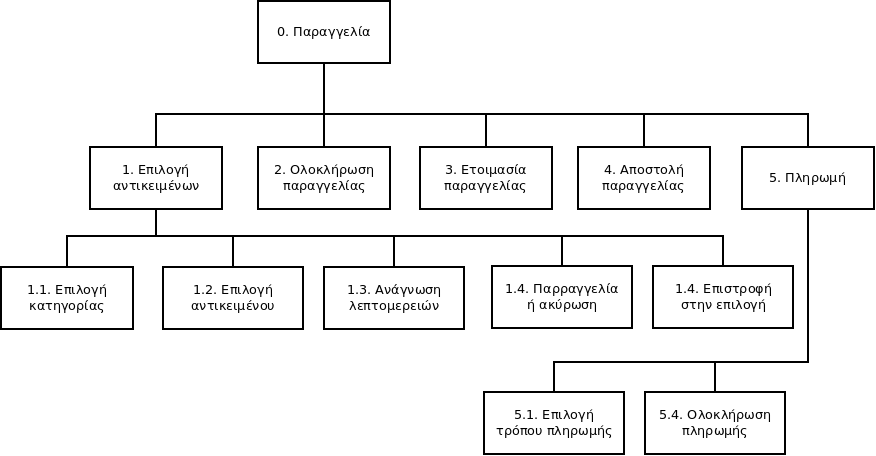
\includegraphics{images/paraggelia.png}}
\caption{Η ιεραρχική ανάλυση εργασιών για την πραγματοποίηση μίας παραγγελίας.}
\label{fig:task_analysis:paraggelia}
\end{center}
\end{figure}

\subsection{Ρύθμιση της πισίνας-τάφρου}

Η εργασία "Ρύθμιση της πισίνας-τάφρου" μπορεί να αναλυθεί ως εξής:

\begin{enumerate}
\setcounter{enumi}{-1}
\item Ρύθμιση της πισίνας-τάφρου
\item Έλεγχος για άνρθωπο
  \begin{enumerate}[label*=\arabic*.]
  \item Αν υπάρχει άνθρωπος μέσα στην πισίνα τότε ελέγχουμε και την ώρα
  \item Αν και οι δύο παραπάνω συνθήκες ισχύουν τότε ενεργοποιείται ο συναγερμός 
  \end{enumerate}
\item Ρύθμιση της στάθμης της πισίνας
  \begin{enumerate}[label*=\arabic*.]
  \item Επιλογή της στάθμης από τον χρήστη
  \item Αλλαγή της στάθμης της πισίνας
  \end{enumerate}
\item Ρύθμιση της θερμοκρασίας της πισίνας
  \begin{enumerate}[label*=\arabic*.]
  \item Επιλογή της θερμοκρασίας από τον χρήστη
  \item Έλεγχος της θερμοκρασίας ότι δεν υπερβαίνει κάποια όρια
  \item Αλλαγή της θερμοκρασίας της πισίνας
  \end{enumerate}
\end{enumerate}

Συνοπτικά η ιεραρχική ανάλυση εργασιών για την πραγματοποίηση μίας παραγγελίας φαίνεται και στο σχήμα \ref{fig:task_analysis:pisina}.

\begin{figure}
\begin{center}
\resizebox*{16.5cm}{!}{
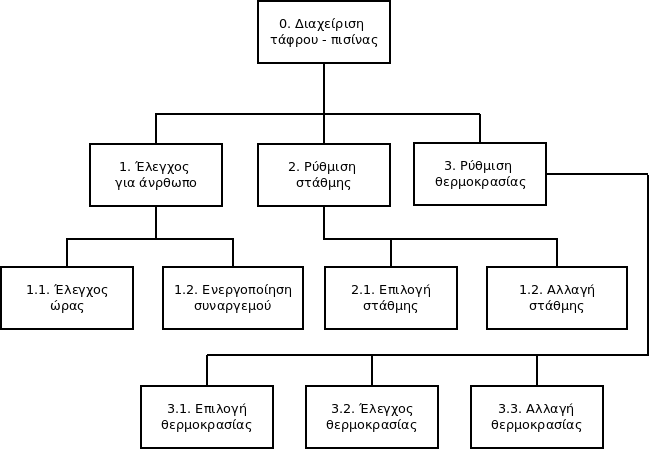
\includegraphics{images/pisina.png}}
\caption{Η ιεραρχική ανάλυση εργασιών για το την ρύθμιση της πισίνας-τάφρου.}
\label{fig:task_analysis:pisina}
\end{center}
\end{figure}

\subsection{Άνοιγμα πόρτας της πισίνας-τάφρου}

Η εργασία "Άνοιγμα πόρτας της πισίνας-τάφρου" μπορεί να αναλυθεί ως εξής:




Συνοπτικά η ιεραρχική ανάλυση εργασιών για την πραγματοποίηση μίας παραγγελίας φαίνεται και στο σχήμα \ref{fig:task_analysis:porta}.

\begin{figure}
\begin{center}
\resizebox*{16.5cm}{!}{
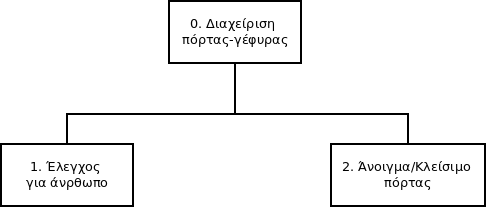
\includegraphics{images/porta.png}}
\caption{Η ιεραρχική ανάλυση εργασιών για το άνοιγμα της πόρτας της πισίνας-τάφρου.}
\label{fig:task_analysis:porta}
\end{center}
\end{figure}



\section{Σχεδιασμός}

Εδώ να βάλουμε την λογική πίσω από την κάθε οθόνη της εφαρμογής και πως λειτουργεί


\section{Υλοποίηση και επαλήθευση}

Εδώ να αναφέρουμε για τον κώδικα

\section{Ενσωμάτωση-Τεκμηρίωση}

Ιδέα δεν έχω

\section{Συντήρηση}

Ιδέα δεν έχω

\phantomsection \label{Βιβλιογραφία}
\addcontentsline{toc}{section}{Βιβλιογραφία}
%\mtcaddchapter[Βιβλιογραφία] % Λόγω του minitoc
\bibliographystyle{plain}
\bibliography{references}

\newpage

\end{document}

